\documentclass{article}
\usepackage{graphicx}

\title{Advanced Machine Learning 1}
\author{Divij Singh}
\date{04/02/19}


\begin{document}

	\maketitle
	
	\section{Q1}
(a)\\
Key:\\
Blue - Data\\
Red - Degree 1\\
Green - Degree 5\\
Yellow - Degree 10\\
Purple - Degree 50\\

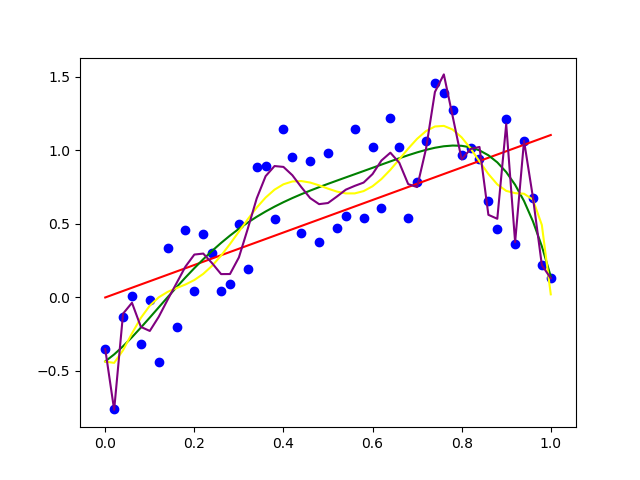
\includegraphics[scale = 0.75]{1.png}
\\\\\\\\
(b)\\
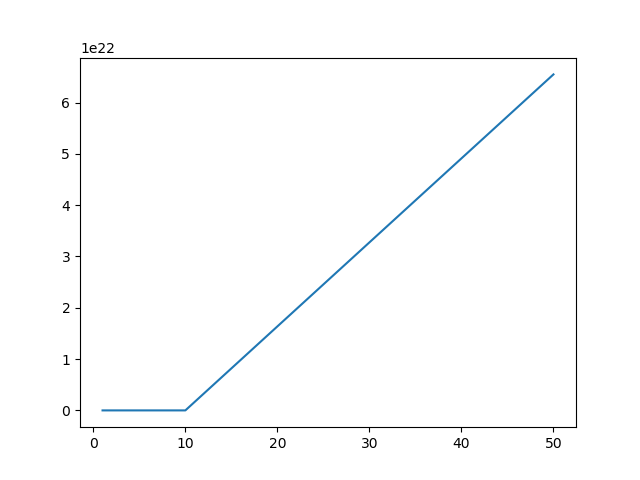
\includegraphics[scale = 0.75]{2.png}
\\
(c)\\
As the degree of the polynomial increases, the MSE increases exponentially.\\
This is due to the fact that at higher polynomials, the model is getting overfit, resulting in wildly innacurate predictions.\\
(d)\\
Key:\\
Red - MSE\\
Blue - Variance\\
Green - Squared Bias\\
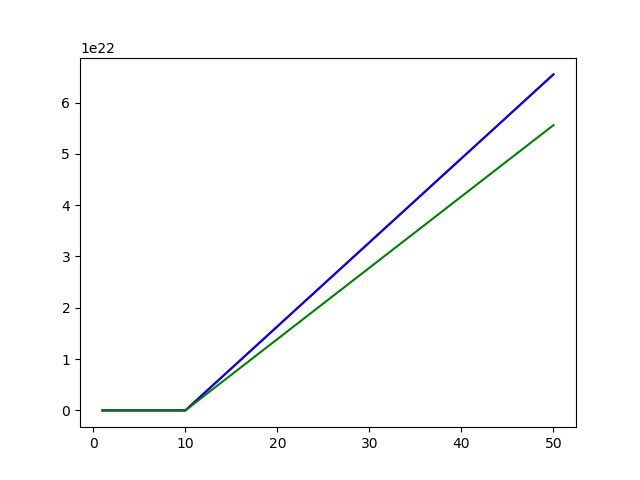
\includegraphics[scale = 0.75]{3.png}
\\
The variance is the same as the MSE, likely due to the overfitting.\\
(e)\\
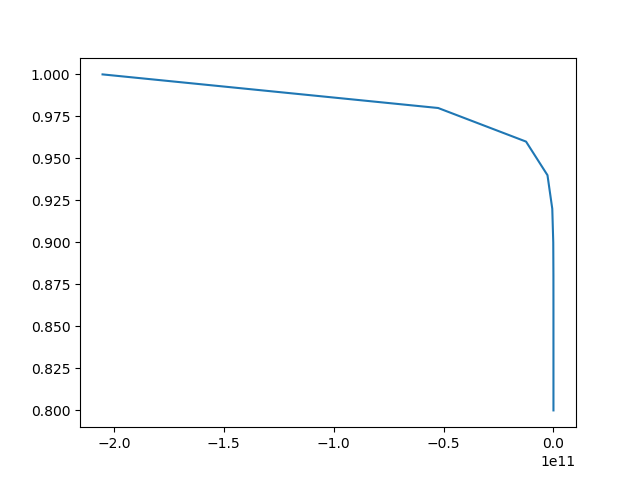
\includegraphics[scale = 0.75]{4.png}\\
This estimator is wildly innacurate, going so far as to double back on itself, whereas the invidual estimators had a consistent line pattern. This is likely due to the overfitting of data.\\
(f)\\
I would expect the estimator to function worse than either of the three estimators did individually.
\end{document}